\documentclass{article}
\usepackage{tikz}
\usepackage{pdfpages}
\usepackage{parskip}
\usepackage{amsmath}
\usepackage[margin=.6in]{geometry}

\begin{document}
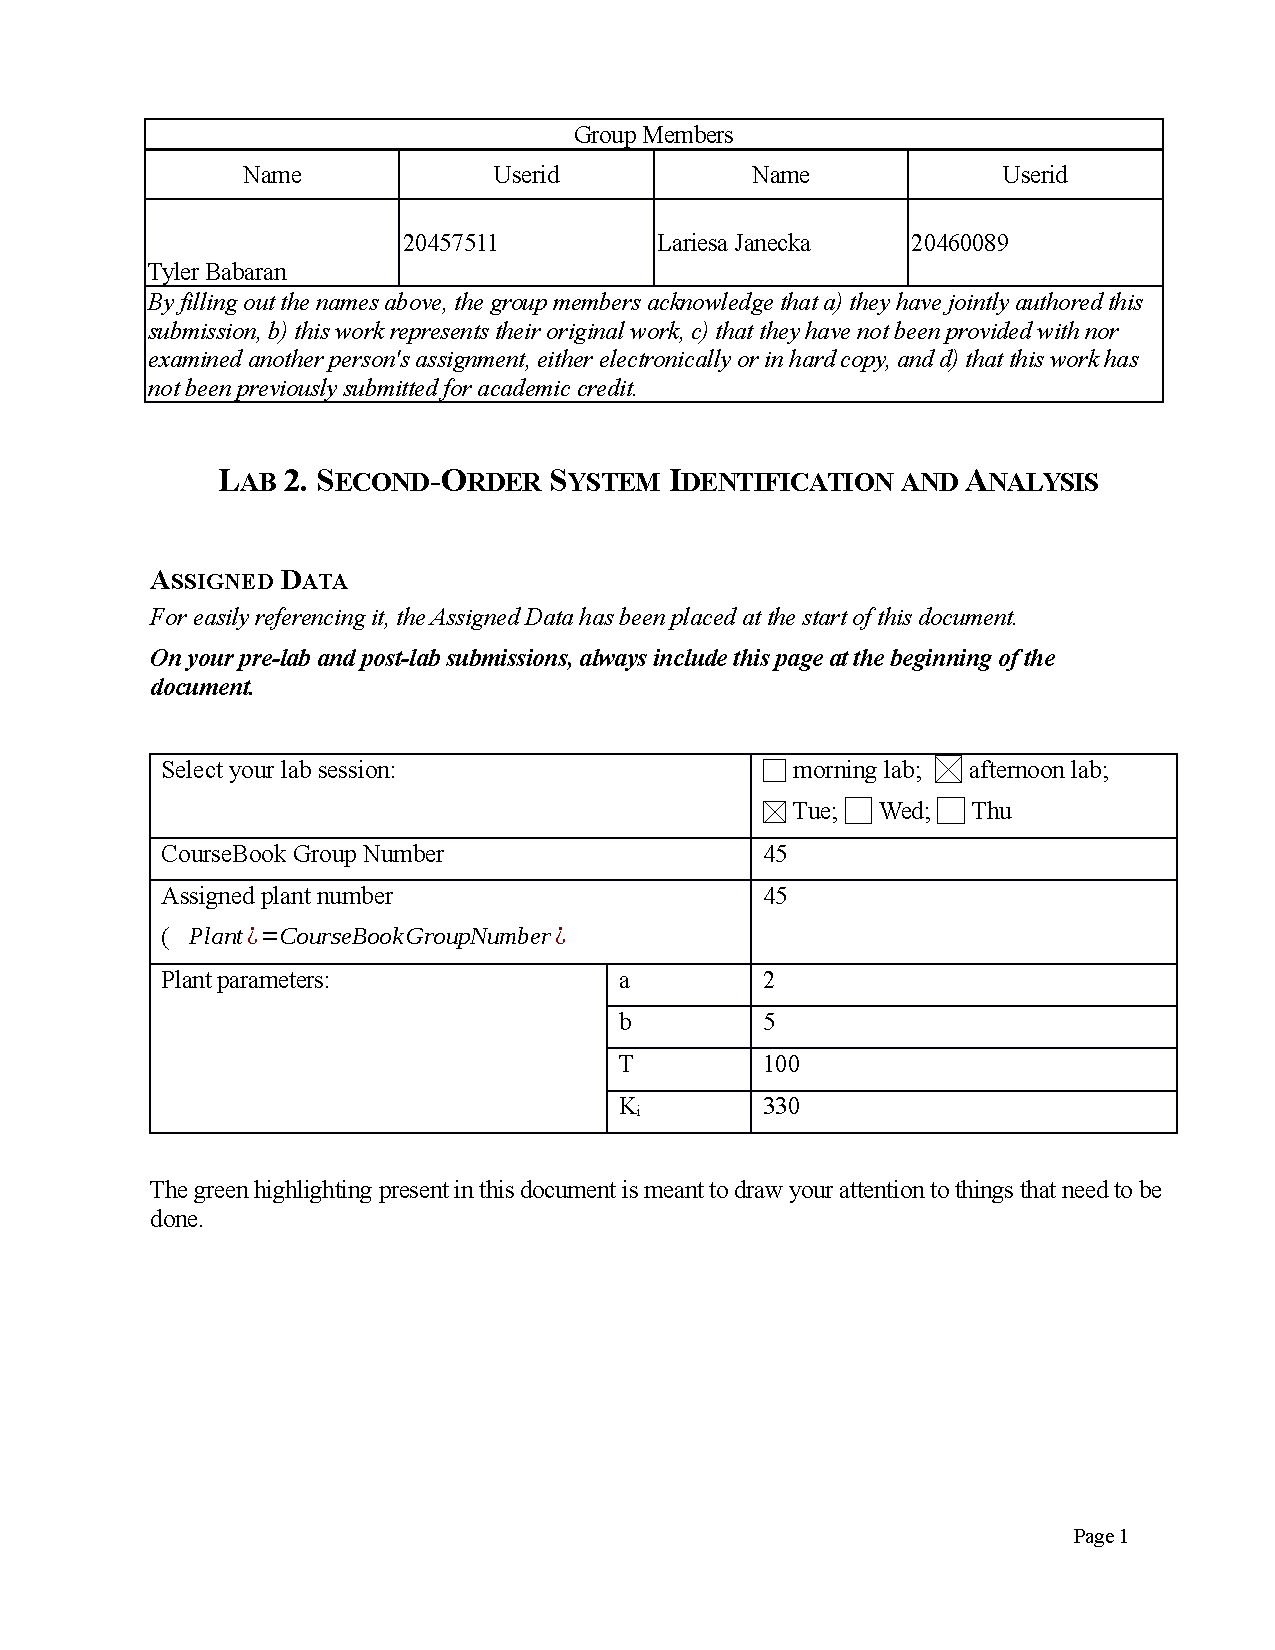
\includepdf[pages={1}]{page1.pdf}
\section*{Section 4.1} % (fold)
\label{sec:section_4_1}

\begin{table}[ht]
\centering
    \begin{tabular}{|c|c|c|c|c|}
        \hline
        $T_p$(s) & $c_{max}$ (V) & $c_{ss}$(V) & $T_r$(s) & $T_s$(s)\\
        \hline
        8.22E-003 & 1.48 & 1 & 3.01E-003 & 3.364E-002\\
        \hline
    \end{tabular}
    \caption{Response specifications - experimental values}
\end{table}

\begin{figure}[ht]
\centering
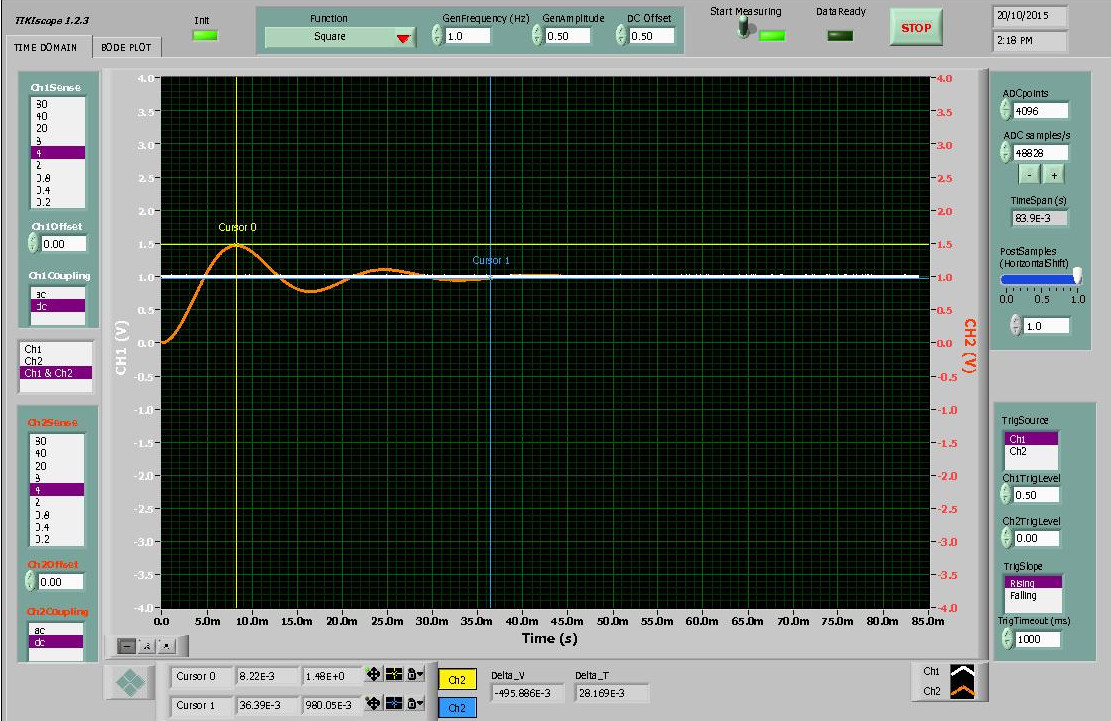
\includegraphics[width=7in]{4_1.jpg}
\caption{Second order underdamped}
\end{figure}

Calculations for table 2:

Using the formula for overshoot
\begin{align*}
    OS &= e^{\frac{-\zeta\pi}{\sqrt{1-\zeta^2}}}\\
    0.48 &= e^{\frac{-\zeta\pi}{\sqrt{1-\zeta^2}}}\\
    \ln {0.48} &= \frac{-\zeta\pi}{\sqrt{1-\zeta^2}}\\
    \ln^2 {0.48} &= \frac{\zeta^2\pi^2}{1-\zeta^2}\\
    \ln^2 {0.48} \times (1-\zeta^2) &= \zeta^2\pi^2\\
    \ln^2 {0.48} &= \zeta^2 \times (\pi^2 +\ln^2 {0.48}) \\
    \zeta &= \sqrt{\frac{\ln^2 {0.48}}{\pi^2 +\ln^2 {0.48}}} \\
    \zeta &=  0.2275\\
\end{align*}

Using the formula for peak time
\begin{align*}
    T_p &= \frac{\pi}{\omega_n\sqrt{1-\zeta^2}}\\
    \omega_n &= \frac{\pi}{T_p\sqrt{1-\zeta^2}}\\
    \omega_n &= \frac{\pi}{0.00822\sqrt{1-\zeta^2}}\\
    \omega_n &= \frac{382.93}{\sqrt{1-\zeta^2}}\\
    \omega_n &= \frac{382.93}{\sqrt{1-0.2275}}\\
    \omega_n &= 435.68\\
\end{align*}


\begin{table}[ht]
\centering
    \begin{tabular}{|c|c|c|c|c|c|}
        \hline
        $T_p$(s) & $c_{max}$ (V) & $c_{ss}$(V) & OS(\%) & $\zeta$ & $\omega_n$(rad/s)\\
        \hline
        8.22E-003 & 1.48 & 1 & 48 & 0.2275 & 435.68\\
        \hline
    \end{tabular}
    \caption{System identification data and results}
\end{table}

\paragraph{Discussing Table 2}

Prelab values: zeta = 0.2462 omega = 406.20

Experimental values: zeta = 0.2275 omega = 435.68

The experimental values differed from the theoretical values calculated in the prelab by around 8\%. Errors may have stemmed from inaccurate graph reading when recording experimental values, or by small rounding errors during mathematical calculations for experimental and theoretical values.

% section section_4_1 (end)

\section*{Section 4.2} % (fold)
\label{sec:section_4_2}

\begin{figure}[ht]
\centering
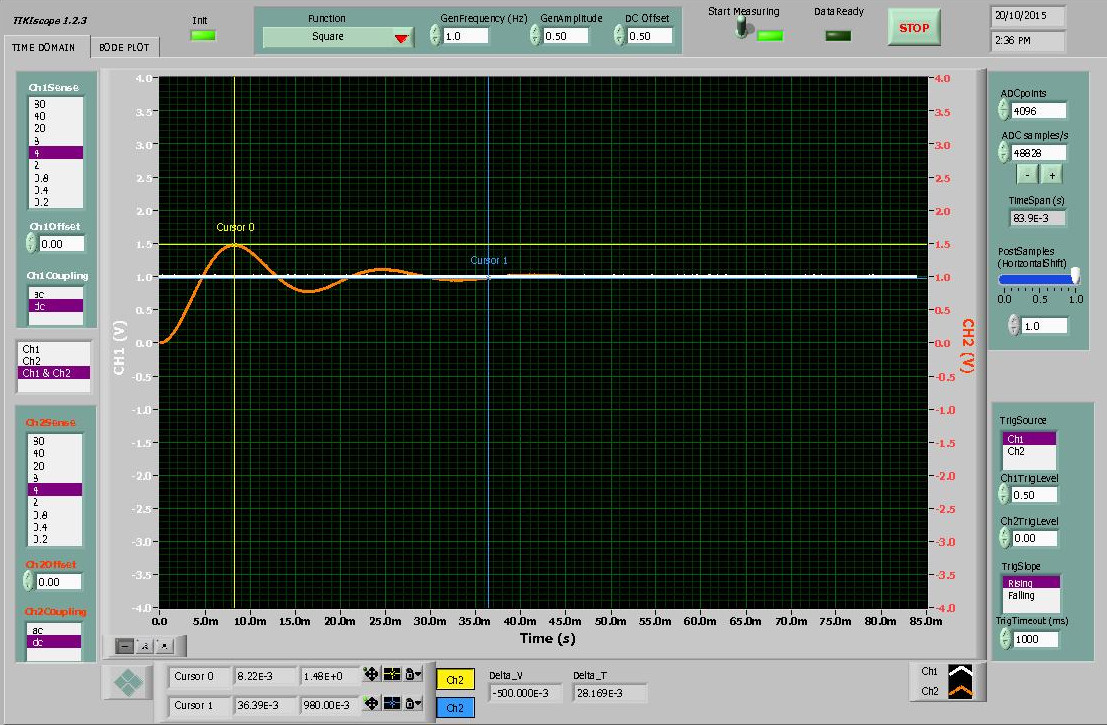
\includegraphics[width=7in]{4_2.jpg}
\caption{Open-loop step response with K=1}
\end{figure}

\begin{table}[ht]
\centering
    \begin{tabular}{|c|c|c|c|c|}
        \hline
        $K_p$ & $T_p$(s) & $y_{max}$(V) & $y_{ss}$(V) & OS(\%)\\
        \hline
        1 &8.2E-003 & 1.48 & 1 & 48\\
        \hline
        1.3 & 8.17E-003 & 1.98 & 1.33 & 49\\
        \hline
        1.66 & 8.27E-003 & 2.47 & 1.66 & 49\\
        \hline
        2 &8.17E-003 & 2.93 & 2 & 47\\
        \hline
    \end{tabular}
    \caption{Open-loop step response values for Kp=variable}
\end{table}

\paragraph{Discussing Table 3}

\textbf{Peak Value}: This increased with Kp. This fits control theory as the peak value is the highest oscillation above the steady state value, since the steady state value is increasing without $\zeta$ changing this value should rise as well.

\textbf{Steady state}: As Kp increases the steady state value increases to match the Kp value. This fits with control theory as the output for G(S) has a steady state value of 1, experimentally verified. For the open loop system the output should be equal to $G(S)\times K\times K_p$ (as they are all in series) and since K stayed at 1 for all experiments the output increase was proportional to Kp.

\textbf{Overshoot and Peak time}: These values did not change much. This fits control theory as the equations for overshoot and peak time are proportional to $\zeta$ and $\omega_n$ which do not vary with with K or Kp in the open-loop system.


\begin{figure}[ht]
\centering
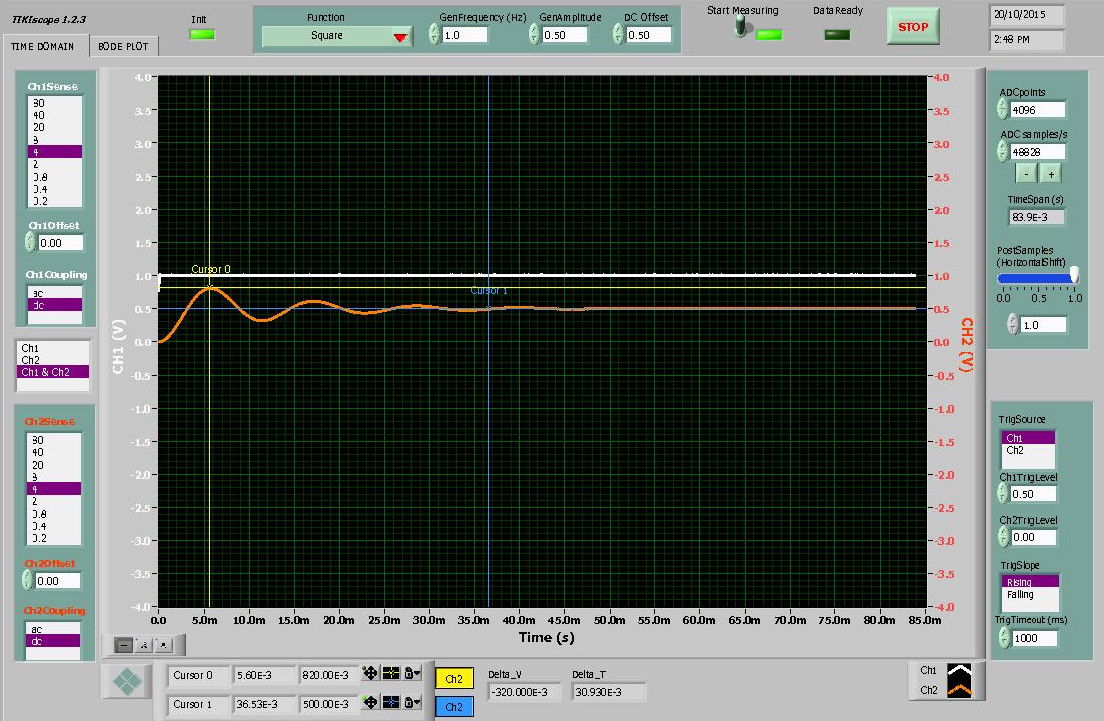
\includegraphics[width=7in]{4_2b.jpg}
\caption{Closed-loop step response with K=1}
\end{figure}
TODO: FIGURE OUT STEADY STATE ERROR FOR TABLE 3
\begin{table}[ht]
\centering
    \begin{tabular}{|c|c|c|c|c|c|}
        \hline
        $K_p$ & $T_p$(s) & $y_{max}$(V) & $y_{ss}$(V) & $e_{ss}$ & OS(\%)\\
        \hline
        1 & 5.6E-003 & 0.82 & 0.5 & & 64\\
        \hline
        1.3 & 5.2E-003 & 0.93 & 0.57 & & 63\\
        \hline
        1.66 & 4.92E-003 & 1.03 & 0.64 & & 62\\
        \hline
        2 & 4.5E-003 & 1.12 & 0.68 & & 65\\
        \hline
    \end{tabular}
    \caption{Closed-loop step response values for Kp=variable}
\end{table}

\paragraph{Discussing Table 4}

\textbf{Peak Value and Steady State value}: These values are increasing with Kp. Due to control theory our system output with the increase of Kp from 1 is:
\begin{align*}
      Y(S) = \frac{K_pH(S)}{1 + K_pH(S)}
  \end{align*}
As Kp increases in the above equation the output will also increase is what causes the increase in the peak value and the steady state value.

\textbf{Overshoot}: The overshoot does not change much. This is due to the steady state and peak value increasing by the same ratio. We can also see that this value will not change because it is related to $\zeta$ which has not changed.

\textbf{Peak Time}: The peak time is decreasing as Kp increases
TODO: FIGURE THIS OUT LATER


TODO: CHECK THAT THIS IS LEGAL
CALCULATE ZETA AND OMEGA N FOR OPEN AND CLOSED LOOP AND COMPARE WITH THEORETICAL
Using the formula for overshoot
\begin{align*}
    \zeta &= \sqrt{\frac{\ln^2 {OS}}{\pi^2 +\ln^2 {OS}}} \\
    \zeta &= \sqrt{\frac{\ln^2 {0.64}}{\pi^2 +\ln^2 {0.64}}} \\
    \zeta &=  0.14\\
\end{align*}

Using the formula for peak time
\begin{align*}
    \omega_n &= \frac{\pi}{T_p\sqrt{1-\zeta^2}}\\
    \omega_n &= \frac{\pi}{0.0056\sqrt{1-0.14^2}}\\
    \omega_n &= 572.21\\
\end{align*}

Open loop values
Theoretical: zeta = 0.2462 omega = 406.20

Experimental values: zeta = 0.2275 omega = 435.68


Adjusted value is k=1.04


\begin{table}[ht]
\centering
    \begin{tabular}{|c|c|c|c|c|}
        \hline
        & Low-freq gain (dB) & Experimental bw (rad/s) & Theor or sim bw (rad/s) & Error (\%)\\
        \hline
        Open-loop & 0.5 & 589 & & \\
        \hline
        Closed-loop & -5.8 & 850 & & \\
        \hline
    \end{tabular}
    \caption{Bandwidth (bw) measurement results}
\end{table}

DISCUSS EFFECTS OF CLOSING THE LOOP ON FREQUENCY RESPONSE

WHY IS IT DESIRABLE TO CHANGE BANDWIDTH

\begin{figure}[ht]
\centering
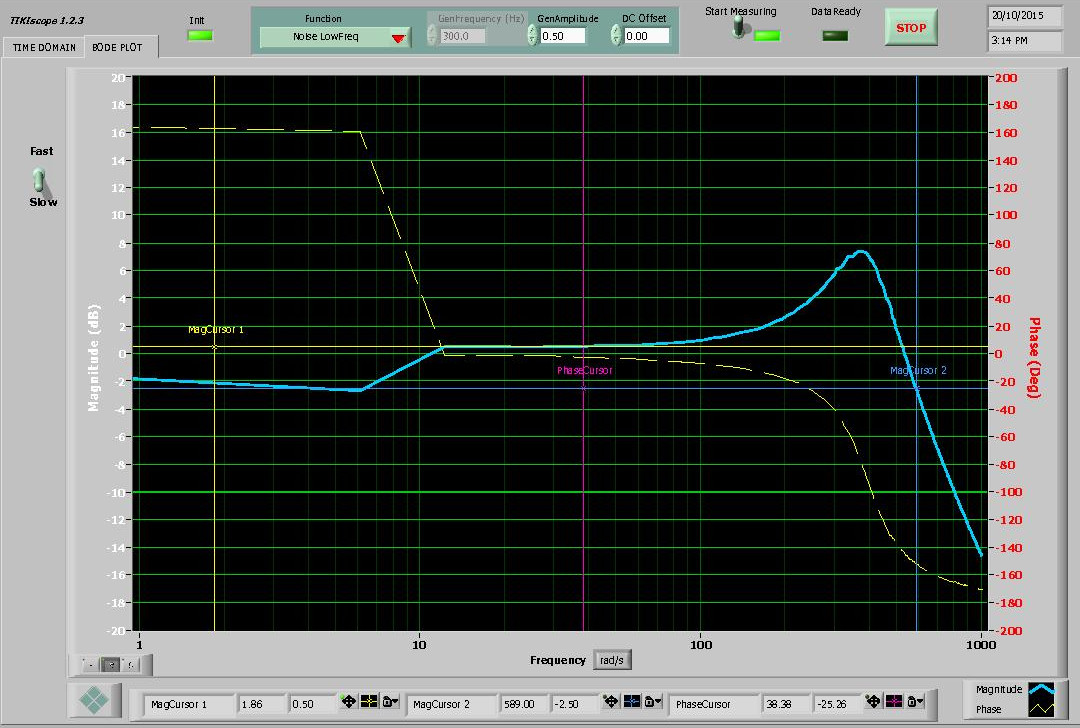
\includegraphics[width=7in]{4_2c(open).jpg}
\caption{Open-loop frequency response}
\end{figure}

\begin{figure}[ht]
\centering
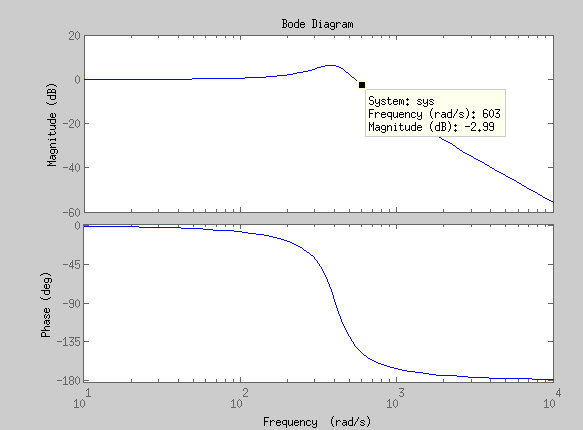
\includegraphics[width=7in]{4_2c(open)_matlab.jpg}
\caption{Matlab open-loop frequency response}
\end{figure}

\begin{figure}[ht]
\centering
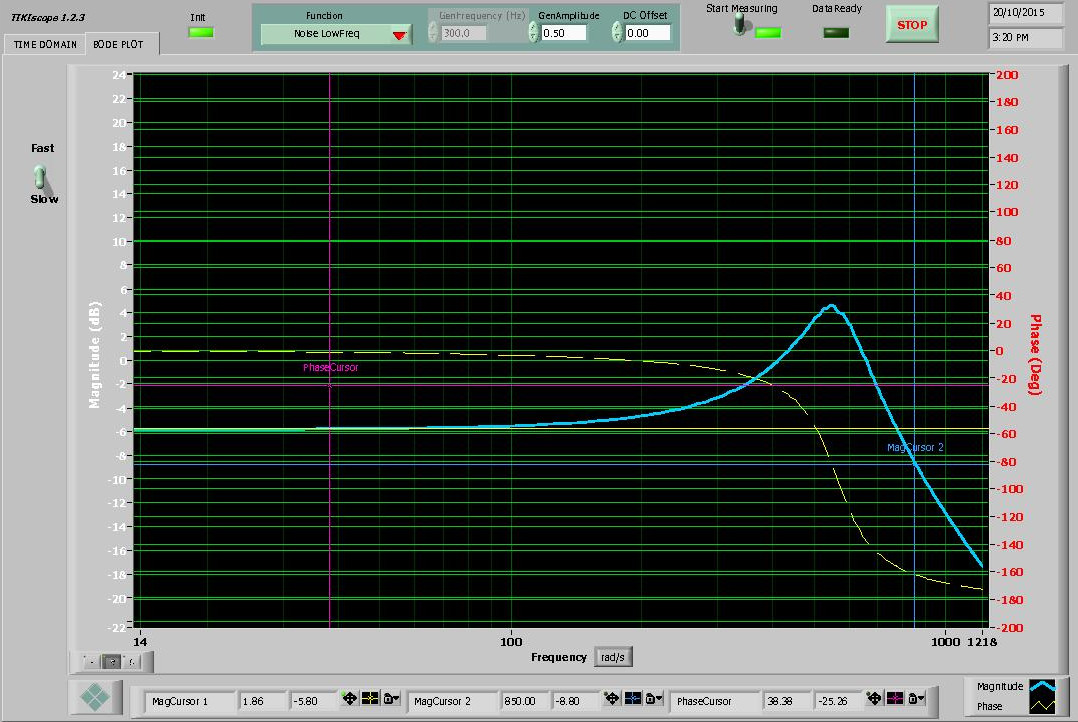
\includegraphics[width=7in]{4_2c(closed).jpg}
\caption{Closed-loop frequency response}
\end{figure}

\begin{figure}[ht]
\centering
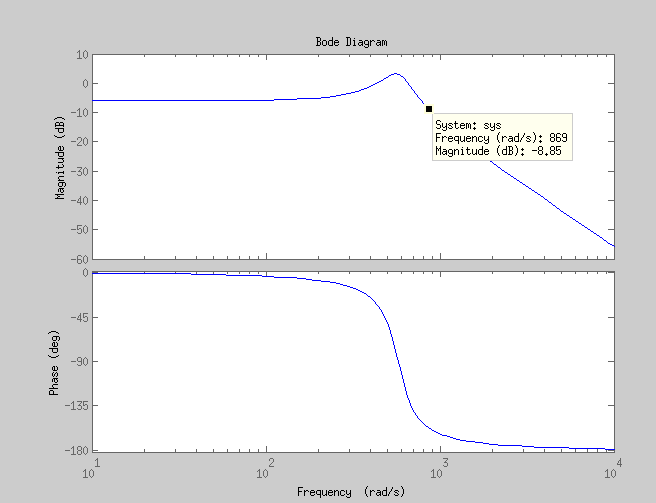
\includegraphics[width=7in]{4_2c(closed)_matlab.jpg}
\caption{Matlab closed-loop frequency response}
\end{figure}


% section section_4_2 (end)

\section*{Section 4.3} % (fold)
\label{sec:section_4_3}


\begin{figure}[ht]
\centering
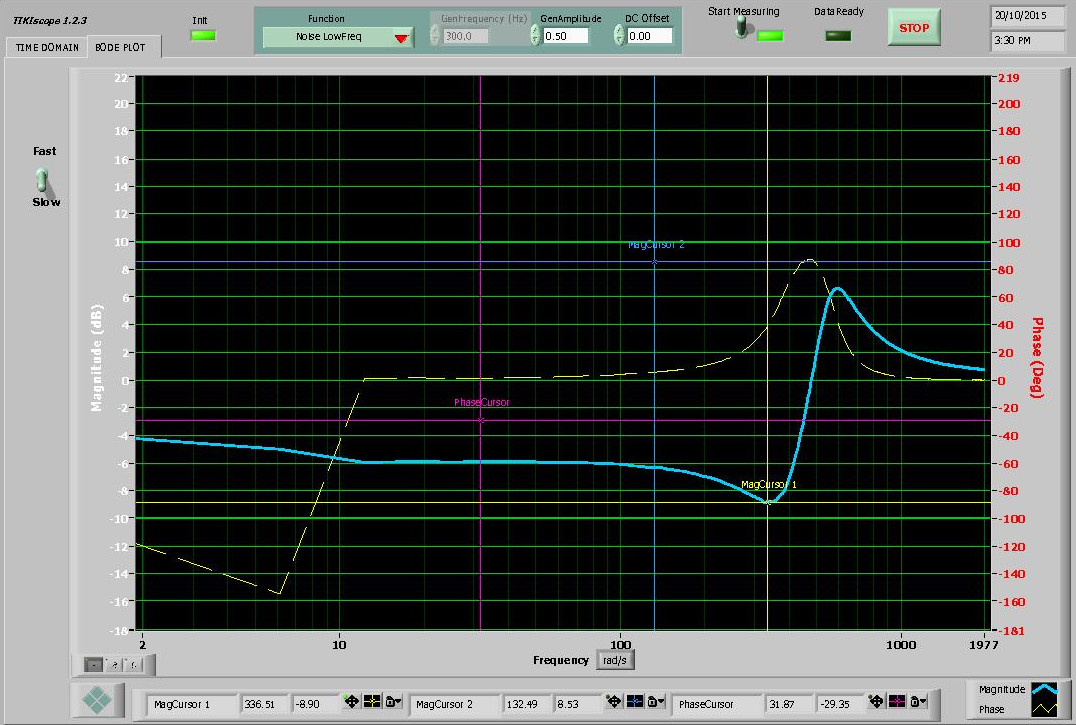
\includegraphics[width=7in]{4_3.jpg}
\caption{Frequency response response with disturbance}
\end{figure}
Comment qualitatively on which frequency ranges present better disturbance rejection

\begin{figure}[ht]
\centering
\includegraphics[width=7in]{4_3_matlab.jpg}
\caption{Frequency response response with disturbance in Matlab}
\end{figure}

% section section_4_3 (end)


\end{document}




